% Name: U-Net
% Description: The U-Net for image segmentation, sketched: an encoder that halves the resolution and doubles the channels at each level, a decoder that undoes it, and skip connections between matching levels.
% Tags: U-Net, segmentation, encoder-decoder, skip connection

\usetikzlibrary{arrows.meta}

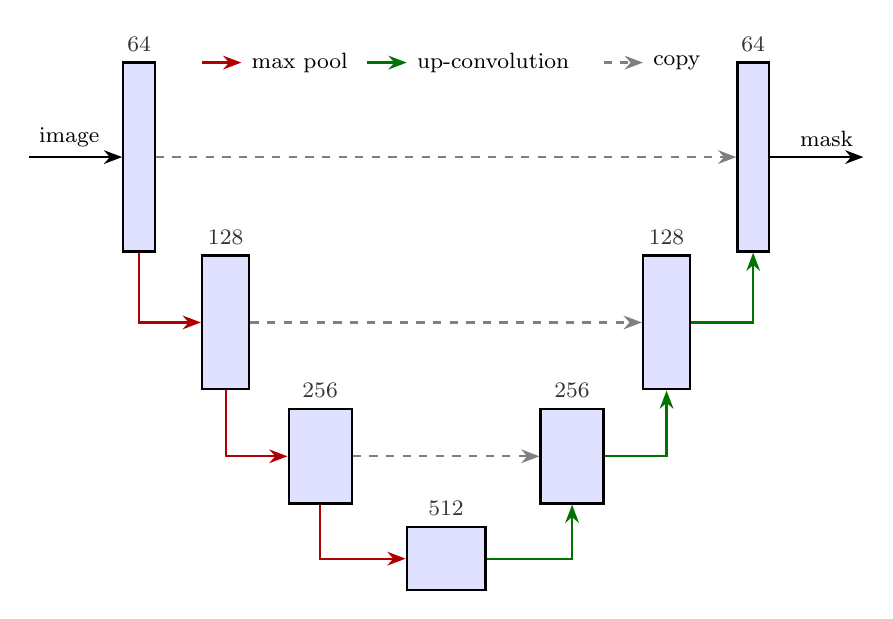
\begin{tikzpicture}[>={Stealth}, thick, every node/.style={font=\footnotesize},
    down/.style={->, red!70!black}, up/.style={->, green!45!black}, skip/.style={->, gray, dashed}]
  % Each block: name, center x, center y, width (grows with channels), height (shrinks with resolution), channels.
  \foreach \n/\x/\y/\w/\h/\c in {e0/0.6/0/0.4/2.4/64, e1/1.7/-2.1/0.6/1.7/128, e2/2.9/-3.8/0.8/1.2/256, b/4.5/-5.1/1/0.8/512,
      d2/6.1/-3.8/0.8/1.2/256, d1/7.3/-2.1/0.6/1.7/128, d0/8.4/0/0.4/2.4/64}
    \node[draw, fill=blue!12, minimum width=\w cm, minimum height=\h cm, inner sep=0pt, label={[gray!40!black]above:\c}] (\n) at (\x,\y) {};
  \draw[down] (e0) |- (e1);
  \draw[down] (e1) |- (e2);
  \draw[down] (e2) |- (b);
  \draw[up] (b) -| (d2);
  \draw[up] (d2) -| (d1);
  \draw[up] (d1) -| (d0);
  \foreach \l in {0, 1, 2} \draw[skip] (e\l) -- (d\l);
  \draw[->] (-0.8,0) node[above right] {image} -- (e0);
  \draw[->] (d0) -- (9.8,0) node[above left] {mask};
  % The legend.
  \draw[down] (1.4,1.2) -- ++(0.5,0) node[right, black] {max pool};
  \draw[up] (3.5,1.2) -- ++(0.5,0) node[right, black] {up-convolution};
  \draw[skip] (6.5,1.2) -- ++(0.5,0) node[right, black] {copy};
\end{tikzpicture}
